\section{Distribución Normal Estándar -- La función $Q(z)$}\label{app:cola gaussiana}

En todo el libro, las probabilidades de error se expresan en términos de la función $Q(z)$, la cola de la distribución Normal estándar definida en \eqref{eq:def cola gaussiana}:
\begin{equation*}
    Q(z) = \p{Z>z} = \int_z^\infty \frac{1}{\sqrt{2\pi}} \e^{-\frac{s^2}{2}} ds, \qquad Z\sim\mathcal{N}(0,1).
\end{equation*}
Si $X\sim\mathcal{N}(\mu,\sigma^2)$, normalizando se obtiene $\p{X>x} = Q\left(\frac{x-\mu}{\sigma}\right)$. De la simetría de la densidad Gaussiana se deducen además las propiedades:
\begin{equation*}
    Q(0) = \frac{1}{2}, \qquad Q(-z) = 1-Q(z).
\end{equation*}

La función $Q$ no tiene expresión cerrada, pero se encuentra implementada en casi todos los paquetes de software. Para $z\gg 1$ vale además la siguiente aproximación:
\begin{equation}\label{eq:aprox Q}
    Q(z) \approx \frac{1}{\sqrt{2\pi}z}\e^{-\frac{z^2}{2}}.
\end{equation}
Esta aproximación muestra que $Q(z)$ decae esencialmente como $\e^{-z^2/2}$: por eso pequeños aumentos en el argumento (es decir, en la relación señal a ruido) producen reducciones de varios órdenes de magnitud en la probabilidad de error. La Figura \ref{fig:funcion Q} muestra la función $Q(z)$ en escala logarítmica.

\begin{figure}
    \begin{center}
        \begin{tikzpicture}
        \begin{semilogyaxis}[
            width=0.8\textwidth, height=.8\textheight,
            xmin=0, xmax=7, ymin=1e-12, ymax=1,
            xlabel={$z$}, ylabel={$Q(z)$},
            xtick distance=1,
            minor x tick num=4,
            grid=both,
            major grid style={line width=0.6pt, draw=gray!60},
            minor grid style={line width=0.2pt, draw=gray!25},
            ]
            \addplot[teal, very thick] coordinates {(0.00,5.0000e-01) (0.10,4.6017e-01) (0.20,4.2074e-01) (0.30,3.8209e-01) (0.40,3.4458e-01) (0.50,3.0854e-01) (0.60,2.7425e-01) (0.70,2.4196e-01) (0.80,2.1186e-01) (0.90,1.8406e-01) (1.00,1.5866e-01) (1.10,1.3567e-01) (1.20,1.1507e-01) (1.30,9.6800e-02) (1.40,8.0757e-02) (1.50,6.6807e-02) (1.60,5.4799e-02) (1.70,4.4565e-02) (1.80,3.5930e-02) (1.90,2.8717e-02) (2.00,2.2750e-02) (2.10,1.7864e-02) (2.20,1.3903e-02) (2.30,1.0724e-02) (2.40,8.1975e-03) (2.50,6.2097e-03) (2.60,4.6612e-03) (2.70,3.4670e-03) (2.80,2.5551e-03) (2.90,1.8658e-03) (3.00,1.3499e-03) (3.10,9.6760e-04) (3.20,6.8714e-04) (3.30,4.8342e-04) (3.40,3.3693e-04) (3.50,2.3263e-04) (3.60,1.5911e-04) (3.70,1.0780e-04) (3.80,7.2348e-05) (3.90,4.8096e-05) (4.00,3.1671e-05) (4.10,2.0658e-05) (4.20,1.3346e-05) (4.30,8.5399e-06) (4.40,5.4125e-06) (4.50,3.3977e-06) (4.60,2.1125e-06) (4.70,1.3008e-06) (4.80,7.9333e-07) (4.90,4.7918e-07) (5.00,2.8665e-07) (5.10,1.6983e-07) (5.20,9.9644e-08) (5.30,5.7901e-08) (5.40,3.3320e-08) (5.50,1.8990e-08) (5.60,1.0718e-08) (5.70,5.9904e-09) (5.80,3.3157e-09) (5.90,1.8175e-09) (6.00,9.8659e-10) (6.10,5.3034e-10) (6.20,2.8232e-10) (6.30,1.4882e-10) (6.40,7.7688e-11) (6.50,4.0160e-11) (6.60,2.0558e-11) (6.70,1.0421e-11) (6.80,5.2310e-12) (6.90,2.6001e-12) (7.00,1.2798e-12)};
        \end{semilogyaxis}
        \end{tikzpicture}
    \end{center}
    \caption{La función $Q(z)$ en escala logarítmica.}\label{fig:funcion Q}
\end{figure}

En la práctica, suele interesar el problema inverso: dado un objetivo de probabilidad de error, qué argumento $z$ se necesita. La siguiente tabla resume algunos valores útiles.
\begin{center}
    \begin{tabular}{c|ccccccccc}
        $Q(z)$ & $10^{-1}$ & $10^{-2}$ & $10^{-3}$ & $10^{-4}$ & $10^{-5}$ & $10^{-6}$ & $10^{-7}$ & $10^{-8}$ & $10^{-9}$ \\ \hline
        $z$ & $1.28$ & $2.33$ & $3.09$ & $3.72$ & $4.26$ & $4.75$ & $5.20$ & $5.61$ & $6.00$
    \end{tabular}
\end{center}
Por ejemplo, para lograr $P_e = Q(z) = 10^{-6}$ se requiere $z\approx 4.75$, es decir, que el margen de ruido normalizado $d/\sigma_N$ (ver Observación \ref{rem:margen ruido}) sea aproximadamente $4.75$.
